% The comment below tells Rubber to compile the .dot files.
%
% rubber: module graphics
% rubber: rules rules.ini

\documentclass{beamer}

\usetheme{default}

\usepackage{helvet}
\usecolortheme{seagull}         % white on black

\usepackage[utf8]{inputenc}
\PassOptionsToPackage{hyphens}{url}\usepackage{hyperref,xspace,multicol}
\usepackage[absolute,overlay]{textpos}
\usepackage{tikz}
\usetikzlibrary{arrows,shapes,trees,shadows,positioning}
\usepackage{fancyvrb}           % for \Verb

% Remember the position of every picture.
\tikzstyle{every picture}+=[remember picture]

\tikzset{onslide/.code args={<#1>#2}{%
  \only<#1>{\pgfkeysalso{#2}} % \pgfkeysalso doesn't change the path
}}

% Colors.
\definecolor{guixred1}{RGB}{226,0,38}  % red P
\definecolor{guixorange1}{RGB}{243,154,38}  % guixorange P
\definecolor{guixyellow}{RGB}{254,205,27}  % guixyellow P
\definecolor{guixred2}{RGB}{230,68,57}  % red S
\definecolor{guixorange2}{RGB}{236,117,40}  % guixorange S
\definecolor{guixtaupe}{RGB}{134,113,127} % guixtaupe S
\definecolor{guixgrey}{RGB}{91,94,111} % guixgrey S
\definecolor{guixblue1}{RGB}{38,109,131} % guixblue S
\definecolor{guixblue2}{RGB}{10,50,80} % guixblue S
\definecolor{guixgreen1}{RGB}{133,146,66} % guixgreen S
\definecolor{guixgreen2}{RGB}{157,193,7} % guixgreen S

\setbeamerfont{title}{size=\huge}
\setbeamerfont{frametitle}{size=\huge}

% White-on-black color theme.
\setbeamercolor{structure}{fg=guixorange1,bg=black}
\setbeamercolor{title}{fg=white,bg=black}
\setbeamercolor{date}{fg=guixorange1,bg=black}
\setbeamercolor{frametitle}{fg=white,bg=black}
\setbeamercolor{titlelike}{fg=white,bg=black}
\setbeamercolor{normal text}{fg=white,bg=black}
\setbeamercolor{alerted text}{fg=guixyellow,bg=black}
\setbeamercolor{section in toc}{fg=white,bg=black}
\setbeamercolor{section in toc shaded}{fg=white,bg=black}
\setbeamercolor{subsection in toc}{fg=guixorange1,bg=black}
\setbeamercolor{subsection in toc shaded}{fg=white,bg=black}
\setbeamercolor{subsubsection in toc}{fg=guixorange1,bg=black}
\setbeamercolor{subsubsection in toc shaded}{fg=white,bg=black}
\setbeamercolor{frametitle in toc}{fg=white,bg=black}
\setbeamercolor{local structure}{fg=guixorange1,bg=black}

\newcommand{\highlight}[1]{\alert{\textbf{#1}}}

\title{Reproducible Software Deployment with GNU~Guix}

\author{Ludovic Courtès}
\date{\small{Inria Rennes Bretagne Atlantique, November 2015}}

\setbeamertemplate{navigation symbols}{} % remove the navigation bar

\AtBeginSection[]{
  \begin{frame}
    \frametitle{}
    \tableofcontents[currentsection]
  \end{frame} 
}


\newcommand{\screenshot}[1]{
  \begin{frame}[plain]
    \begin{tikzpicture}[remember picture, overlay]
      \node [at=(current page.center), inner sep=0pt]
        {\includegraphics[width=\paperwidth]{#1}};
    \end{tikzpicture}
  \end{frame}
}


\begin{document}

\maketitle

\setbeamercolor{normal text}{bg=guixblue2}
\begin{frame}
  \Huge{\textbf{The difficulty of keeping software environments under
      control.}}
\end{frame}
\setbeamercolor{normal text}{fg=white,bg=black}

\begin{frame}[plain]
  \Huge{\#1. Upgrades are hard.}
\end{frame}

\screenshot{images/debian-upgrade-warning}
\screenshot{images/debian-upgrade-instructions}

\begin{frame}[plain]
  \Huge{\#2. Stateful system management is intractable.}
\end{frame}

\begin{frame}[plain, fragile]
  \begin{overlayarea}{\textwidth}{8cm}
  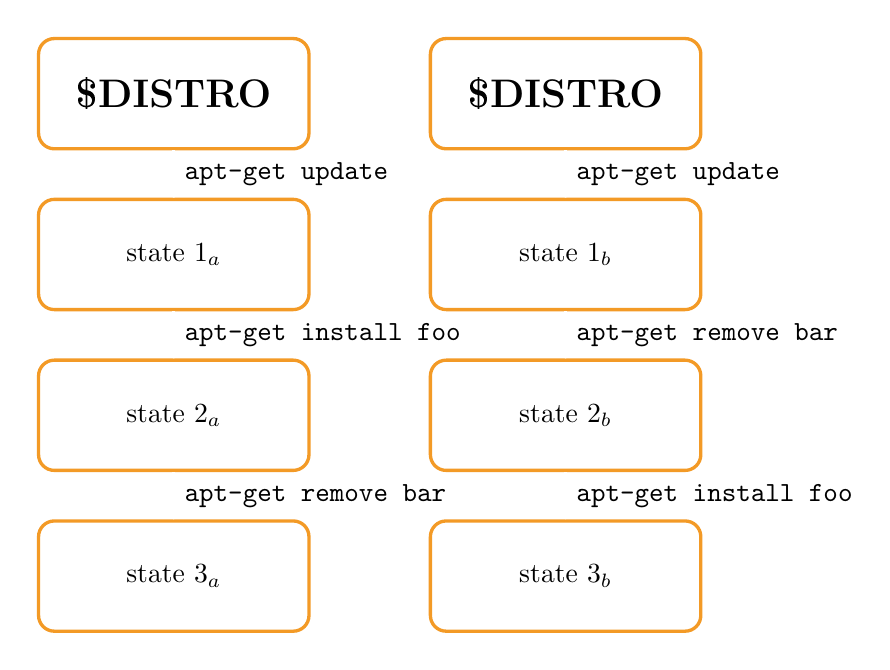
\begin{tikzpicture}[stylish/.style = {
                        draw=guixorange1, very thick,
                        fill=white, text=black, text width=3.2cm,
                        rounded corners=2mm, minimum height=1.4cm,
                        text centered
                      }]
    \matrix[row sep=6mm, column sep=1.5cm] {
      \node(inita)[stylish]{\textbf{\Large{\$DISTRO}}};
      & \node(initb)[stylish]{\textbf{\Large{\$DISTRO}}};
      \\

      \node<2->(state1a)[stylish]{state $1_a$};
      & \node<2->(state1b)[stylish]{state $1_b$};
      \\

      \node<3->(state2a)[stylish]{state $2_a$};
      & \node<3->(state2b)[stylish]{state $2_b$};
      \\

      \node<4->(state3a)[stylish]{state $3_a$};
      & \node<4->(state3b)[stylish]{state $3_b$};
      \\
    };

    \path[->, very thick, draw=white]<2->
      (inita) edge node[right]{\texttt{apt-get update}} (state1a);
    \path[->, very thick, draw=white]<3->
      (state1a) edge node[right]{\texttt{apt-get install foo}} (state2a);
    \path[->, very thick, draw=white]<4->
      (state2a) edge node[right]{\texttt{apt-get remove bar}} (state3a);
    
    \path[->, very thick, draw=white]<2->
      (initb) edge node[right]{\texttt{apt-get update}} (state1b);
    \path[->, very thick, draw=white]<3->
      (state1b) edge node[right]{\texttt{apt-get remove bar}} (state2b);
    \path[->, very thick, draw=white]<4->
      (state2b) edge node[right]{\texttt{apt-get install foo}} (state3b);

  \end{tikzpicture}
  \end{overlayarea}

  \begin{tikzpicture}[overlay]
    \node<5>[rounded corners=4, text centered,
          fill=guixorange1, text width=3cm,
          inner sep=5mm, opacity=.75, text opacity=1,
          drop shadow={opacity=0.5}] at (5, 4) {
            \textbf{\Huge{= ?}}
          };
  \end{tikzpicture}
\end{frame}

\begin{frame}[plain]
  \Huge{\#3. It's worse than this.}
\end{frame}

\screenshot{images/package-managers-cropped}

\begin{frame}[plain]
  \Huge{It's worse, really.}
\end{frame}

\begin{frame}
  \Large{``Let's Package jQuery: A Javascript Packaging Dystopian
    Novella'' by Chris Webber}
  \\[2.cm]
  
  \url{http://dustycloud.org/blog/javascript-packaging-dystopia/}
\end{frame}

\begin{frame}[plain]
  \LARGE{\textbf{Giving up?}}
  \\[1.0cm]
  \uncover<2->{$\rightarrow$ ``app bundles'' (Docker images)}
\end{frame}

\screenshot{images/docker-security}

% TODO: http://www.vitavonni.de/blog/201503/2015031201-the-sad-state-of-sysadmin-in-the-age-of-containers.html

\begin{frame}[plain]
  \begin{tikzpicture}[remember picture, overlay]
    \node [at=(current page.center), inner sep=0pt]
          {
\includegraphics[height=\paperheight]{images/hope-hero}};
  \end{tikzpicture}
\end{frame}

%% \section{Functional Package Management}

\setbeamercolor{normal text}{bg=guixblue2}
\begin{frame}[plain]
  \Huge{\textbf{Functional package management.}}
\end{frame}
\setbeamercolor{normal text}{fg=white,bg=black}

\begin{frame}[plain]
  \Large{
    $\texttt{openmpi} = f(\texttt{hwloc}, \texttt{gcc}, \texttt{make},\texttt{coreutils})$
    
    \uncover<2->{$\texttt{hwloc} = g(\texttt{pciaccess}, \texttt{gcc}, \texttt{make}, \texttt{coreutils})$}

    \uncover<3->{$\texttt{gcc} = h(\texttt{make}, \texttt{coreutils}, \texttt{gcc}_0)$}
    
    \uncover<3->{\textrm{...}}
  }

  \uncover<1>{\large{where $f =$ \texttt{./configure \&\& make \&\& make install}}}

  \begin{tikzpicture}[overlay]
    \node<4->[fill=guixorange1, text=black, text opacity=1, opacity=.7,
          rounded corners=2mm, inner sep=5mm] at (5, 1) {
            \textbf{\Large{the complete DAG is captured}}
          };
  \end{tikzpicture}
\end{frame}

\begin{frame}
  \Large{
    \begin{itemize}
    %% \item<3-> \textit{Caching Function Calls Using Precise Dependencies}
    %%   (``Vesta''), Heydon et al., 2000
    \item \textit{A Safe and Policy-Free System for Software
      Deployment}, Dolstra et al., 2003\\ \alert{\textbf{Nix}},
      \url{http://nixos.org/nix/}
    \item \textit{Functional Package Management with Guix}, Courtès,
      2013
    \end{itemize}
  }
\end{frame}

\begin{frame}[fragile]
  \begin{semiverbatim}
(define hello
  (\alert{package}
   (name "hello")
   (version "2.10")
   (source (\alert{origin}
            (method url-fetch)
            (uri (string-append
                  "mirror://gnu/\textrm{...}/hello-" version
                  ".tar.gz"))
            (sha256 (base32 "0wqd\textrm{...}dz6"))))
   (\alert{build-system} gnu-build-system)
   (synopsis "Hello, world!")
   (description "Produce a friendly greeting.")
   (home-page "http://www.gnu.org/software/hello/")
   (license gpl3+)))
  \end{semiverbatim}

  % \begin{tikzpicture}[overlay]
  %   \node[rounded corners=4, text centered,
  %         fill=guixorange1, text width=3cm,
  %         inner sep=3mm, rotate=-5, opacity=.75, text opacity=1,
  %         drop shadow={opacity=0.5},
  %         at=(current page.center)] {
  %           \textbf{\large{Emacs + Geiser demo!}}
  %         };
  % \end{tikzpicture}
\end{frame}

\begin{frame}[fragile]{}
  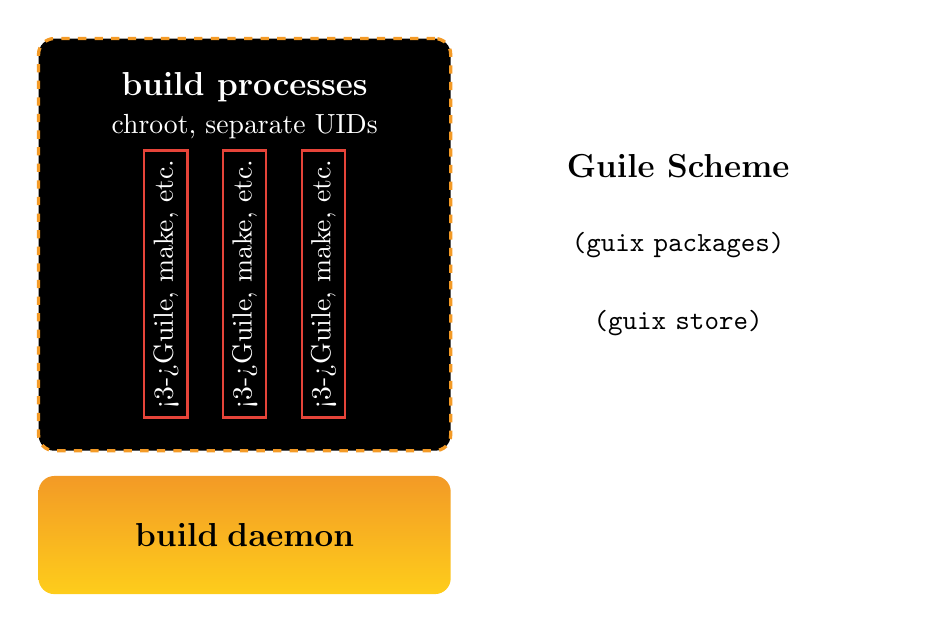
\begin{tikzpicture}[tools/.style = {
                        text width=35mm, minimum height=4cm,
                        text centered,
                        rounded corners=2mm,
                        fill=white, text=black
                      },
                      tool/.style = {
                        fill=white, text=black, text width=3cm,
                        text centered
                      },
                      daemon/.style = {
                        rectangle, text width=50mm, text centered,
                        rounded corners=2mm, minimum height=15mm,
                        top color=guixorange1,
                        bottom color=guixyellow,
                        text=black
                      },
                      builders/.style = {
                        draw=guixorange1, very thick, dashed,
                        fill=black, text=white, text width=5cm,
                        rounded corners=2mm,
                      },
                      builder/.style = {
                        draw=guixred2, thick, rectangle,
                        fill=black, text=white,
                        rotate=90
                      }]
    \matrix[row sep=3mm, column sep=1cm] {
      \node(builders)[builders, text height=5cm]{}
          node[fill=black, text=white] at (0, 2) {\large{\textbf{build processes}}}
          node[fill=black, text=white] at (0, 1.5) {chroot, separate UIDs}
          node[builder, onslide=<1-2>{black}] at (-1,-0.5) {\alert<3->{Guile}, make, etc.}
          node[builder, onslide=<1-2>{black}] at ( 0,-0.5) {\alert<3->{Guile}, make, etc.}
          node[builder, onslide=<1-2>{black}] at ( 1,-0.5) {\alert<3->{Guile}, make, etc.}; &
      \node[tools]{}
          node[fill=white, text=black] at (0, 1) {\large{\textbf{Guile Scheme}}}
          node[tool] at (0, 0) {\texttt{(guix packages)}}
          node(client)[tool] at (0, -1) {\texttt{(guix store)}};
      \\

      \node(daemon)[daemon]{\large{\textbf{build daemon}}}; &
      &
      \\
    };
  \end{tikzpicture}

  \begin{tikzpicture}[overlay]
    \path[very thick, draw=guixorange1]<2->
      (client.south) edge [out=-90, in=0, ->] node[below, sloped]{RPCs} (daemon.east);
    \path[->, very thick, draw=guixorange1]<3->
      (daemon) edge (builders);
  \end{tikzpicture}
\end{frame}

\begin{frame}[fragile]
  %% \frametitle{Bit-Reproducible Builds$^*$}
  %% \framesubtitle{$^*$ almost!}

  \begin{semiverbatim}
\$ guix build hello
\uncover<2->{/gnu/store/\tikz[baseline]{\node[anchor=base](nixhash){\alert<2>{h2g4sf72\textrm{...}}};}-hello-2.10}

\uncover<3->{\$ \alert<3>{guix gc --references /gnu/store/\textrm{...}-hello-2.10}
/gnu/store/\textrm{...}-glibc-2.22
/gnu/store/\textrm{...}-gcc-4.9.3-lib
/gnu/store/\textrm{...}-hello-2.10
}
  \end{semiverbatim}

  \begin{tikzpicture}[overlay]
    \node<1>(labelnixhash) [fill=white, text=black] at (current page.center) {%
      \Large{\textbf{isolated build}: chroot, separate name spaces, etc.}
    };

    \node<2>(labelnixhash) [fill=white, text=black] at (4cm, 2cm) {%
      hash of \textbf{all} the dependencies};
    \path[->]<2>(labelnixhash.north) edge [bend left, in=180, out=-45] (nixhash.south);

    \draw<4-> (-10pt, 105pt) [very thick, color=guixorange2, rounded corners=8pt]
      arc (10:-50:-50pt and 110pt);
    \node<4->[fill=white, text=black, text opacity=1, opacity=.7,
          rounded corners=2mm, inner sep=5mm]
      at (7, 2) {\textbf{\Large{(nearly) bit-identical for everyone}}};
    %% \node<5>[fill=white, text=black, text opacity=1, opacity=.7,
    %%       rounded corners=1mm, inner sep=3mm]
    %%   at (8, 1) {\url{http://reproducible.debian.net}};
  \end{tikzpicture}

\end{frame}

\begin{frame}[fragile]

  \begin{semiverbatim}
\$ guix package -i gcc-toolchain coreutils sed grep
\textrm{...}

\$ eval `guix package --search-paths`
\textrm{...}

\$ guix package --manifest=my-software.scm
\textrm{...}
  \end{semiverbatim}

  \begin{tikzpicture}[overlay]
    \node[rounded corners=4, text centered,
          fill=guixorange1, text width=3cm,
          inner sep=3mm, rotate=5, opacity=.75, text opacity=1,
          drop shadow={opacity=0.5}] at (5, 4) {
            \textbf{\large{demo}}
          };
  \end{tikzpicture}
\end{frame}

\begin{frame}[fragile]
  \Huge{Want your PhD student to hack on GNUnet?}
  \\[2cm]
  \uncover<2->{\Large{A simple matter of installing the deps, right?}}
\end{frame}

\begin{frame}[plain]
  \begin{tikzpicture}[remember picture, overlay]
    \node [at=(current page.center), inner sep=0pt]
          {\includegraphics[width=\paperwidth]{images/gnunet-graph}};
  \end{tikzpicture}
\end{frame}


\begin{frame}[fragile]
  \begin{semiverbatim}
\$ guix environment --container gnunet
\textrm{...}

\$ guix environment --ad-hoc python-ipython python-numpy \\
    -E ipython
\textrm{...}

  \end{semiverbatim}
\end{frame}

\screenshot{images/ci-jenkins-cropped}

\setbeamercolor{normal text}{bg=guixblue2}
\begin{frame}[plain]
  \Huge{\textbf{Whole-system deployment.}}
\end{frame}
\setbeamercolor{normal text}{fg=white,bg=black}

\begin{frame}[fragile]
  \begin{overlayarea}{\textwidth}{8cm}
  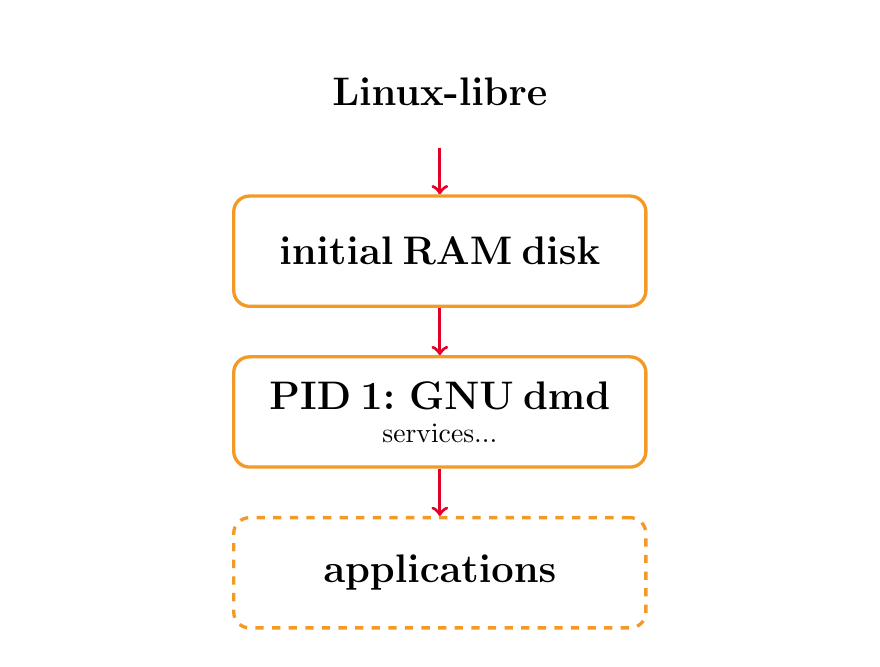
\begin{tikzpicture}[kernel/.style = {
                        text width=10cm, minimum height=1.4cm,
                        text centered,
                        rounded corners=2mm,
                        fill=white, text=black
                      },
                      userland/.style = {
                        draw=guixorange1, very thick,
                        fill=white, text=black, text width=5cm,
                        rounded corners=2mm, minimum height=1.4cm,
                        text centered
                      }]
    \matrix[row sep=6mm, column sep=1cm] {
      \node(kernel)[kernel]{\textbf{\Large{Linux-libre}}};
      \\

      \node<2->(initrd)[userland]{\textbf{\Large{initial RAM disk}}};
      \\

      \node<4->(dmd)[userland]{\textbf{\Large{PID 1: GNU dmd}}
        \\ services...};
      \\

      \node<6->(user)[userland, dashed]{\textbf{\Large{applications}}};
      \\
    };

    \path[->, very thick, draw=guixred1]<2->
      (kernel) edge (initrd);
    \path[->, very thick, draw=guixred1]<4->
      (initrd) edge (dmd);
    \path[->, very thick, draw=guixred1]<6->
      (dmd) edge (user);
    
  \end{tikzpicture}
  \end{overlayarea}

  \begin{tikzpicture}[overlay,
                      guile/.style = {
                         fill=guixyellow, text=black, rotate=30,
                         rounded corners=4mm, text width=3cm,
                         opacity=.75, text opacity=1, text centered,
                         minimum height=1.3cm
                      }]
    \node<3->(labelinitrd) [guile] at (initrd.east) {%
      \Large{Guile}
    };
    \node<5->(labelinitrd) [guile] at (dmd.east) {%
      \Large{Guile}
    };
  \end{tikzpicture}
\end{frame}

\setbeamercolor{normal text}{bg=guixblue2}
\begin{frame}[plain]
  \Huge{\textbf{Trustworthiness.}}
\end{frame}
\setbeamercolor{normal text}{fg=white,bg=black}

\begin{frame}[plain]
  \begin{quotation}
    \noindent
    \Large{Debian’s dirtiest secret:\\
      \noindent
      \textbf{Binary packages \alert{built by developers} are used in
        the archive}}
  \end{quotation}
  \hfill{ --- Lucas Nussbaum, FOSDEM 2015}
\end{frame}

% TODO: CIA's XCode exploit here

\begin{frame}[fragile]
  \frametitle{Transparent binary/source deployment}
  \begin{overlayarea}{\textwidth}{6cm}
    \begin{semiverbatim}
alice@foo\$ \alert{guix package --install=}emacs
The following package will be installed:
   emacs-24.5	/gnu/store/\dots{}-emacs-24.5
\only<1>{
The following files will be \alert{downloaded}:
   /gnu/store/\dots{}-emacs-24.5
   /gnu/store/\dots{}-libxpm-3.5.10
   /gnu/store/\dots{}-libxext-1.3.1
   /gnu/store/\dots{}-libxaw-1.0.11
}\only<2>{
The following files will be \alert{downloaded}:
   /gnu/store/\dots{}-libxext-1.3.1
   /gnu/store/\dots{}-libxaw-1.0.11
The following derivations will be \alert{built}:
   /gnu/store/\dots{}-emacs-24.5.drv
   /gnu/store/\dots{}-libxpm-3.5.10.drv
}
    \end{semiverbatim}
  \end{overlayarea}
\end{frame}

\begin{frame}[plain, fragile, t]
  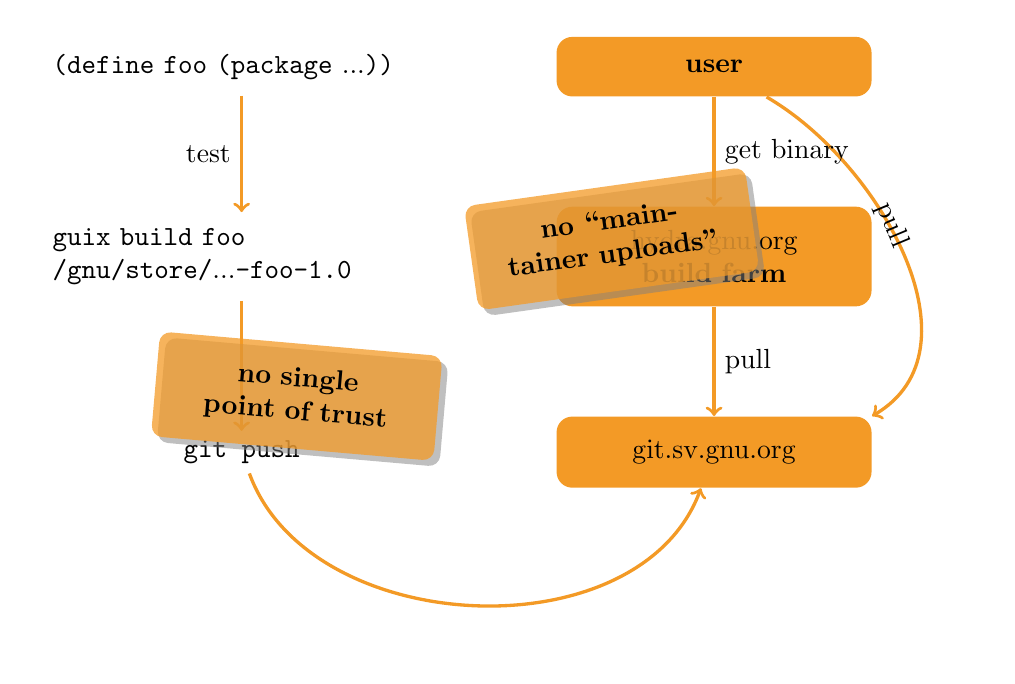
\begin{tikzpicture}[box/.style = {
                         rounded corners=2mm,
                         fill=white, text=black, text width=4.8cm,
                         inner sep=2mm
                      },
                      server/.style = {
                         text centered, rounded corners=2mm,
                         fill=guixorange1, text=black, text width=3.4cm,
                         inner sep=3mm
                      },
                      note/.style = {
                        rounded corners=4, text centered,
                        fill=guixorange1, text width=3cm,
                        inner sep=3mm, rotate=5, opacity=.75, text opacity=1,
                        drop shadow={opacity=0.5}
                      }]
    \matrix[row sep=1.4cm, column sep=1.4cm] {
      \node(def)[box]{\texttt{(define foo (package \textrm{...}))}};
      & \node(user)[server]{\textbf{user}};
      \\
      \node<2->(build)[box]{\texttt{guix build foo}
         \texttt{/gnu/store/\textrm{...}-foo-1.0}};
      & \node<4-5>(hydra)[server]{hydra.gnu.org \textbf{build~farm}};
      \\
      \node<3->(push){\texttt{git push}};
      & \node<3->(savannah)[server]{git.sv.gnu.org}; \\
      \\
    };

    \path[->, very thick, draw=guixorange1]<2->
      (def) edge node[left]{test} (build);
    \path[->, very thick, draw=guixorange1]<3->
      (build) edge (push);
    \path[->, very thick, draw=guixorange1]<3->
      (push) edge[->, in=-110, out=-70] (savannah);
    \path[->, very thick, draw=guixorange1]<4-5>
      (hydra) edge node[right]{pull} (savannah);
    \path[->, very thick, draw=guixorange1]<4-6>
      (user) edge[in=30,out=-30] node[left, sloped]{pull}
      (savannah.north east);
    \path[->, very thick, draw=guixorange1]<5>
      (user) edge node[right]{get binary} (hydra);

    \node<7>[overlay, fill=black, opacity=.8, 
             text height=9cm, text width=11cm,
             at=(current page.center)] {};

    \node<7>[note, rotate=3] at (2,1) {\textbf{no ``maintainer uploads''}};
    \node<7>[note, rotate=-10] at (-2,-1) {\textbf{no single point of trust}};
  \end{tikzpicture}
\end{frame}

\begin{frame}[plain, fragile]
  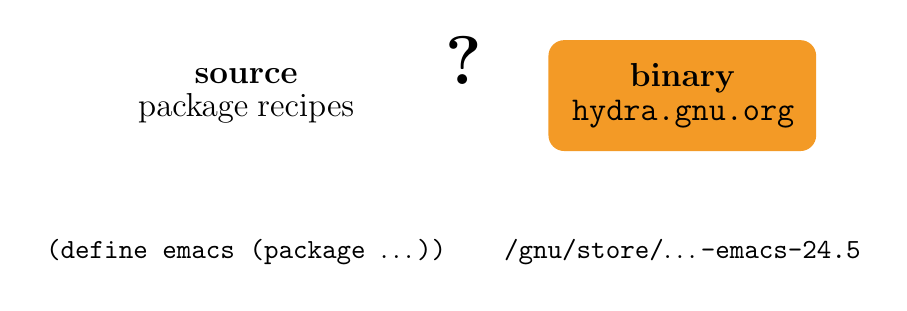
\begin{tikzpicture}[white/.style = {
                         text centered, rounded corners=2mm,
                         fill=white, text=black, text width=2.8cm,
                         inner sep=3mm
                      },
                      orange/.style = {
                         text centered, rounded corners=2mm,
                         fill=guixorange1, text=black, text width=2.8cm,
                         inner sep=3mm
                      }]
    \matrix[row sep=1cm, column sep=0.5cm] {
      \node(source)[white]{\large{\textbf{source}}\\package~recipes};
      & \node(binary)[orange]{\large{\textbf{binary}} \texttt{hydra.gnu.org}};
      \\
      \node{\texttt{(define emacs (\alert{package} \textrm{\dots{}}))}};
      & \node{\texttt{/gnu/store/\textrm{\dots{}}-emacs-24.5}};
      \\
    };

    \path[<->, very thick, draw=white]
      (source) edge node[above]{\Huge{\textbf{?}}} (binary);
  \end{tikzpicture}
\end{frame}

\begin{frame}{The path to greater user control}
  \Large{
  \begin{enumerate}
  \item{ \textbf{Bit-reproducible builds}
    \begin{itemize}
    \item<2-> we have \highlight{isolated build environments}!
    \item<2-> ... but we need builds to be \highlight{deterministic}
    \item<2-> \url{http://reproducible-builds.org}
    \end{itemize}}
  \item{\textbf{No single binary provider}
    \begin{itemize}
    \item<3-> \texttt{guix publish}
    \item<3-> publish over GNUnet? (GSoC 2015)
  \end{itemize}}
  \item \textbf{\alert<4>{Tools for users to challenge binaries}}
  \end{enumerate}
  }
\end{frame}

\begin{frame}[fragile]
  \begin{semiverbatim}
$ \alert{guix challenge} --substitute-urls="http://hydra.gnu.org http://guix.example.org"
\alert{/gnu/store/\dots{}-openssl-1.0.2d contents differ}:
  local hash: 0725l22\dots{}
  http://hydra.gnu.org/\dots{}-openssl-1.0.2d: 0725l22\dots{}
  http://guix.example.org/\dots{}-openssl-1.0.2d: 1zy4fma\dots{}
\alert{/gnu/store/\dots{}-git-2.5.0 contents differ}:
  local hash: 00p3bmr\dots{}
  http://hydra.gnu.org/\dots{}-git-2.5.0: 069nb85\dots{}
  http://guix.example.org/\dots{}-git-2.5.0: 0mdqa9w\dots{}
\alert{/gnu/store/\dots{}-pius-2.1.1 contents differ}:
  local hash: 0k4v3m9\dots{}
  http://hydra.gnu.org/\dots{}-pius-2.1.1: 0k4v3m9\dots{}
  http://guix.example.org/\dots{}-pius-2.1.1: 1cy25x1\dots{}
  \end{semiverbatim}
\end{frame}

%% \begin{frame}
%%   \frametitle{Ken Thompson's attack?}

%%   \begin{itemize}
%%     \item ``Reflections on Trusting Trust'', Ken Thompson
%%     \item ``Countering ... Through Diverse Double Compilation'', David
%%       A. Wheeler
%%   \end{itemize}
%% \end{frame}

\setbeamercolor{normal text}{bg=guixblue2}
\begin{frame}[plain]
  \Huge{\textbf{Status.}}
\end{frame}
\setbeamercolor{normal text}{fg=white,bg=black}

\begin{frame}{Timeline}
  \begin{itemize}
    \item Nov. 2012 --- dubbed GNU
    \item{Jan. 2013 --- \alert{0.1}}
    \item ...
    \item{Apr. 2014 --- \alert{0.6}, signed binaries, \texttt{guix
        system}}
    \item{July 2014 --- \alert{0.7}, \textbf{installable operating
        system}}
    \item ...
    \item{29 Jan. 2015 --- \alert{0.8.1}, \textbf{ARMv7 port}}
    \item ...
    \item Aug. 2015 --- Reproducibility in Parallel Computing Workshop
      (RepPar)
    \item{5 Nov. 2015 --- \alert{0.9.0}, new service framework, etc.}
  \end{itemize}
\end{frame}

\screenshot{images/better}

\begin{frame}{Status}
  \Large{
  \begin{itemize}
    \item full-featured package manager
    \item 2,600+ packages, 4 platforms
    \item \textbf{Guix System Distribution$^\beta$}
    \item binaries at \url{http://hydra.gnu.org}
    \item tooling: auto-update, ``linting'', etc.
    \item l10n: 8 languages!
  \end{itemize}}
\end{frame}

\begin{frame}
  \Large{
    \begin{itemize}
    \item $\approx$25 contributors each month
    \item ... and lots of friendly people!
    \item $\approx$400 commits per month
    \item $\approx$200--500 new packages per release
    \end{itemize}
  }
\end{frame}


\begin{frame}[plain]

  \vspace{0.7cm}
  \Large{
    \begin{itemize}
    \item \textbf{install the distribution}
    \item \textbf{use it}, report bugs, add packages
    \item help with the \textbf{infrastructure} + admin
    \item \textbf{donate} hardware/money
    \item share your \textbf{ideas}!
    \end{itemize}
  }

  \begin{textblock}{5}(7,8)
    \tikz
    \node[overlay, rounded corners=4, text centered,
          minimum size=10mm, fill=guixorange1, text width=5cm,
          inner sep=3mm, rotate=-7, opacity=.75, text opacity=1,
          drop shadow={opacity=0.5}] at (3, 3) {
            \textbf{your help needed!}
          };
  \end{textblock}
\end{frame}


%%%%%%%%%%%%%%%%%%%%%%%%%%%%%%%%%%%%%%%%%%%%%%%%%%%%%%%%%%%%%%%%%%%%%%%%%%%%%%
\begin{frame}[plain]

\vfill{
  \vspace{2.5cm}
  \center{
\includegraphics[width=0.3\textwidth]{images/GuixSD}}\\[1.0cm]
  \texttt{ludo@gnu.org}\hfill{\alert{\url{http://gnu.org/software/guix/}}}
}

\end{frame}

\begin{frame}{}

  \begin{textblock}{12}(2, 8)
    \tiny{
      Copyright \copyright{} 2010, 2012, 2013, 2014, 2015 Ludovic Courtès \texttt{ludo@gnu.org}.\\[3.0mm]
      GNU Guix logo, GFDL, \url{http://gnu.org/s/guix/graphics}

      Copyright of other images included in this document is held by
      their respective owners.
      \\[3.0mm]
      This work is licensed under the \alert{Creative Commons
        Attribution-Share Alike 3.0} License.  To view a copy of this
      license, visit
      \url{http://creativecommons.org/licenses/by-sa/3.0/} or send a
      letter to Creative Commons, 171 Second Street, Suite 300, San
      Francisco, California, 94105, USA.
      \\[2.0mm]
      At your option, you may instead copy, distribute and/or modify
      this document under the terms of the \alert{GNU Free Documentation
        License, Version 1.3 or any later version} published by the Free
      Software Foundation; with no Invariant Sections, no Front-Cover
      Texts, and no Back-Cover Texts.  A copy of the license is
      available at \url{http://www.gnu.org/licenses/gfdl.html}.
      \\[2.0mm]
      % Give a link to the 'Transparent Copy', as per Section 3 of the GFDL.
      The source of this document is available from
      \url{http://git.sv.gnu.org/cgit/guix/maintenance.git}.
    }
  \end{textblock}
\end{frame}

\end{document}

% Local Variables:
% coding: utf-8
% comment-start: "%"
% comment-end: ""
% ispell-local-dictionary: "american"
% compile-command: "rubber --pdf talk.tex"
% End:

%%  LocalWords:  Reproducibility
